\chapter{Keamanan Sistem Email}

{\em Electronic mail} (email\footnote{Dalam bahasa Indonesia sudah ada istilah
{\bf surel} untuk email ini. Dalam buku ini saya masih menggunakan istilah
email.}) masih merupakan salah satu aplikasi yang paling populer di internet.
Bahkan alamat email digunakan sebagai identitas pengguna di internet. Jika Anda
mendaftar ke sebuah layanan, email digunakan sebagai identitas.

Beberapa masalah keamanan terkait dengan sistem email antara lain:
\begin{itemize}
\item disadap ({\em intercept});
\item dipalsukan ({\em forgery});
\item disusupi ({\em intrude});
\item digunakan untuk spamming;
\item mailbomb;
\item mail relay.
\end{itemize}

\section{Komponen Sistem Email}
Sebelum membahas masalah keamanan tersebut ada baiknya kita melihat komponen
dari sebuah sistem mail. Pemahaman tentang komponen ini dibutuhkan untuk
memahami potensi sumber masalah keamanan email.
Sebuah sistem email terdiri dari beberapa komponen;
{\em mail user agent} (MUA),
{\em mail transfer agent} (MTA), dan
{\em mail delivery agent} (MDA).
(Lihat Gambar~\ref{fig:email-topologi}.)

\begin{figure}[ht]
\fbox{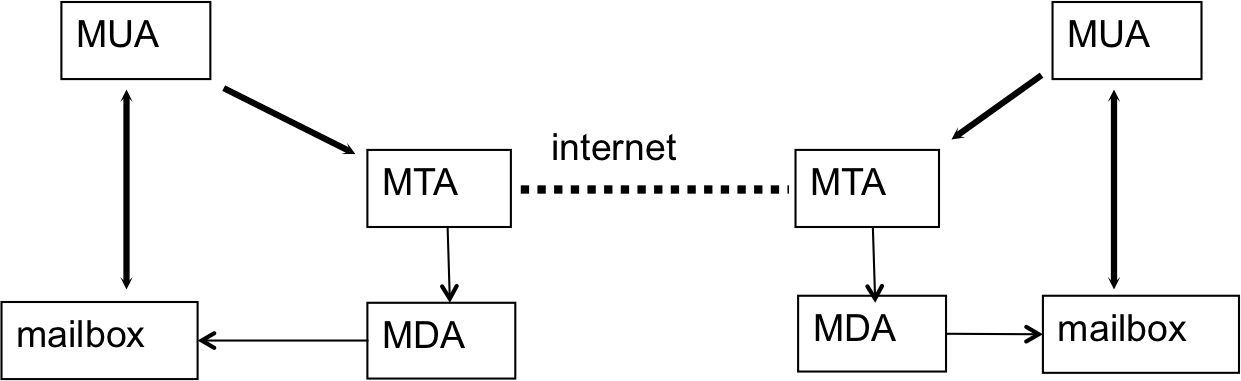
\includegraphics[width=1.0\linewidth]{graphics/email-topologi.png}}
\caption{Topologi Sistem Email}
\label{fig:email-topologi}
\end{figure}

MUA adalah komponen yang berhubungan dengan pengguna. Biasanya MUA adalah yang
kita sebut program email. Contoh dari MUA antara lain adalah Thunderbird,
Outlook, Mac Mail.app, mutt, UNIX mail, pine, dan masih banyak lagi. (Daftar
ini sering berubah.)
Pengguna menggunakan MUA untuk membuat ({\em compose}) dan membaca email.

MTA adalah komponen yang bertugas untuk mengirimkan dan menerima email. Dia
adalah ``pak pos''. MTA menerima berkas email dari MUA dan meneruskannya ke MTA
lainnya dan seterusnya sampai ke MTA yang dituju. Contoh dari MTA antara lain
adalah postfix, sendmail, qmail, Exchange, exim, dan sejenisnya. MTA biasanya
adalah urusan dari administrator.

MDA adalah komponen yang bertugas untuk menyimpan email yang datang ke mailbox
pengguna. Dahulu, MDA ini menjadi bagian dari MTA, tetapi kemudian dipisahkan
karena pemisahan role agar lebih aman. MDA harus menambahkan email yang baru
masuk ke mailbox pengguna. Untuk itu MDA harus memiliki hak untuk menulis ke
mailbox tersebut, dengan kata lain MDA harus dijalankan dengan hak admin atau
{\em super user / root}. Sementara itu MTA tidak harus dijalanakan sebagai admin.

Skenario yang terjadi adalah sebagai berikut. Seorang pengguna (A) membuat
email dengan menggunakan MUA. Setelah email selesai dibuat, email diberikan
kepada MTA untuk disampaikan kepada MTA penerima (B). Kadang MTA yang dituju
tidak langsung dapat diakses tetapi melalui MTA lainnya dahulu.  Sesampainya di
MTA tujuan, email diberikan ke MDA untuk ditambahkan ke mailbox penerima (B).
Penerima (B) tidak harus online ketika email tersebut itu sampai. Ketika
penerima (B) akan membaca email, maka dia akan menggunakan MUA untuk mengakses
mailbox. Jika dia (B) akan membalas, maka digunakan MUA untuk menuliskan
balasannya. Setelah selesai, email balasan diteruskan ke MTA untuk disampaikan
ke MTA tujuan (A).


\section{Standar Email}
Pengguna email memiliki sistem dan konfigurasi yang bervariasi. Masalah
{\em interoprability} merupakan salah satu aspek yang sangat penting. Untuk itu
digunakan RFC (Request For Comments) sebagai standar.

Standar format email didefinisikan oleh RFC 822, ``Standard for the format of 
ARPA Internet text messages.'' (RFC ini sudah digantikan oleh RFC~2822,
``Internet Message Format.'') Pada prinsipnya email dibagi dua bagian; {\bf
header} dan {\bf body}.

\begin{itemize}
   \item {\em Header}. Seperti amplop, berisi informasi tentang alamat pengirim
      yang dituju. Header ini berisi {\em field} yang nantinya digunakan oleh
      MTA untuk mengirimkan ke tujuan.
   \item {\em Body}. Isi surat. Body dipisahkan dari header dengan satu baris
      kosong. 
\end{itemize}

Contoh dari (format) email dapat dilihat sebagai berikut. Perhatikan bahwa
header dan body dipisahkan oleh satu baris kosong. Contoh ini tentu saja
merupakan simplifikasi dari format email sesungguhnya.

\begin{mdframed}
\begin{verbatim}
From: Budi Rahardjo <budi@cert.or.id>
To: br@paume.itb.ac.id
Subject: Kelas EL776 hari ini

Kelas hari ini dibatalkan dan akan digantikan dengan
hari lain.

-- budi
\end{verbatim}
\end{mdframed}

Ada standar {\em field} di header yang mudah terlihat oleh pengguna, yaitu {\em
From}, {\em To}, {\em Subject}, {\em Cc}, dan {\em Bcc}. Padahal ada banyak
{\em field-field} lain yang biasanya terdapat dalam email. Berikut ini contoh
header yang lebih komplit lagi. (Mengenai masing-masing field di header
tersebut akan dibahas lebih lanjut.)

\begin{mdframed}
\begin{verbatim}
Received: from nic.cafax.se (nic.cafax.se [192.71.228.17])
   by alliance.globalnetlink.com (8.9.1/8.9.1) with ESMTP id QAA31830
   for <budi@alliance.globalnetlink.com>; Mon, 26 Mar 2001 16:18:01 -0600
Received: from localhost (localhost [[UNIX: localhost]])
   by nic.cafax.se (8.12.0.Beta6/8.12.0.Beta5) id f2QLSJVM018917
   for ietf-provreg-outgoing; Mon, 26 Mar 2001 23:28:19 +0200 (MEST)
Received: from is1-55.antd.nist.gov (is1-50.antd.nist.gov [129.6.50.251])
   by nic.cafax.se (8.12.0.Beta5/8.12.0.Beta5) with ESMTP id f2QLSGiM018912
   for <ietf-provreg@cafax.se>; Mon, 26 Mar 2001 23:28:17 +0200 (MEST)
Received: from barnacle (barnacle.antd.nist.gov [129.6.55.185])
   by is1-55.antd.nist.gov (8.9.3/8.9.3) with SMTP id QAA07174
   for <ietf-provreg@cafax.se>; Mon, 26 Mar 2001 16:28:14 -0500 (EST)
Message-ID: <04f901c0b63b$16570020$b9370681@antd.nist.gov>
From: "Scott Rose" <scottr@antd.nist.gov>
To: <ietf-provreg@cafax.se>
Subject: confidentiality and transfers
Date: Mon, 26 Mar 2001 16:24:05 -0500
MIME-Version: 1.0
X-Mailer: Microsoft Outlook Express 5.50.4133.2400
Sender: owner-ietf-provreg@cafax.se
Precedence: bulk
\end{verbatim}
\end{mdframed}

Nama {\em field} biasanya berupa satu kata atau jika lebih dari satu kata
disambungkan dengan tanda garis (dash) dan diakhiri dengan tanda titik dua (:).
Isi dari field berupa teks. (Panjang dari teks ini biasanya kurang dari 80
karakter karena merupakan bawaan dari sistem-sistem jaman dahulu.) Jika teks
membutuhkan lebih dari satu baris, maka lanjutannya dapat diletakkan di
bawahnya dengan masuk (indent) menggunakan spasi atau tab.

Selain {\em field} yang sudah standar, kita juga dapat membuat {\em field}
sendiri. Aturannya adalah nama {\em field} tersebut dimulai dengan ``X-''.
Misalnya kita dapat membuat field ``X-catatan:'' yang dapat kita gunakan untuk
menuliskan catatan kecil. Oleh MTA dan MUA, {\em field} tambahan ini akan
diabaikan. Pada contoh sebelumnya dapat dilihat sebuah contoh, yaitu
``X-Mailer:''.

\begin{verbatim}
X-Mailer: Microsoft Outlook Express 5.50.4133.2400
\end{verbatim}

Pemahaman fungsi dari masing-masing field itu dibutuhkan ketika kita akan
melakukan {\em forensic} terhadap email, karena seringkali ada email palsu atau
email-email ancaman. Sebagian besar orang memang tidak tahu keberadaan
field-field tersebut.

Salah satu field yang penting adalah ``Message-ID''. Setiap email memiliki kode
Message-ID yang berbeda-beda (unik). Message-ID ini dibuat oleh MTA ketika dia
mengirimkan email (yang pertama kali). Identitas ini dapat membantu kita dalam
melakukan pelacakan. Sebagai contoh, kita bisa mencari (bertanya) apakah di
berkas catatan (log) di server mail pengirim ada Message-ID tersebut. Ini
sangat bermanfaat dalam penyidikan.

\section{Penyadapan Email}
Email sering dianalogikan dengan surat, padahal email lebih cocok dianalogikan
dengan kartu pos karena dia terbuka dan dapat dibaca. Kartu pos dapat dibaca
oleh orang-orang yang dilewati oleh kartu pos tersebut, misalnya oleh pak pos.
Demikian pula dengan email. Email dapat dibaca pada setiap jalur yang dilewati
oleh email tersebut, misalnya pada MTA.

Pengiriman email antar MTA pada awalnya menggunakan protokol SMTP, Simple Mail
Transfer Protokol (RFC 821). Sesuai dengan namanya, SMTP merupakan protokol
yang sederhana yang tidak memiliki pengamanan terhadap aspek penyadapan. SMTP
menggunakan protokol TCP dan berjalan di atas port 25. Penyadapan port 25 ini
dapat dilakukan dengan menggunakan program {\em sniffer} seperti {\em tcpdump}
dan {\em wireshark}.

Penyadapan email ini dapat dilakukan pada jalur yang dilewati oleh email. Jadi
kita tidak dapat menangkap email yang berada pada segmen jaringan yang berbeda.

Penggunaan {\em tcpdump} untuk menyadap email memang dapat dilakukan, tetapi
data yang diperoleh masih mentah dan harus disambung-sambungkan lagi untuk
mendapatkan email yang tersusun lengkap (dan berurutan). Ada program {\em
mailsnarf} yang dapat melakukan hal tersebut\footnote{Program mailsnarf
terdapat dalam paket {\em dsniff}. Sayangnya paket program ini sudah tidak
dikembangkan lagi. Di berbagai implementasi dari mailsnarf nampaknya tidak
dapat menangkap email lagi. Untuk merakit ulang program ini dibutuhkan skill
yang lumayan.}.

\begin{verbatim}
unix$ mailsnarf > sniffed-mails
\end{verbatim}

Berkas hasil tangkapan {\em mailsnarf} dapat dibuka dengan menggunakan MUA
(program email) yang biasa kita gunakan.

Ada beberapa cara untuk mengamankan email kita dari penyadapan. Yang pertama,
dari sisi pengguna, kita dapat melakukan enkripsi terhadap body email sehingga
meskipun email kita disadap tetapi sang penyadap tidak dapat memperoleh isiny.
Cara ini dapat dilakukan dengan mudah jika kita menggunakan PGP atau GPG.

Cara yang lebih baik adalah dengan menggunakan protokol yang lebih aman. SMTPS,
atau SMTP Secure, merupakan implementasi SMTP yang menggunakan enkripsi. Pada
prinsipnya klien (MTA) tetap menggunakan protokol SMTP tetapi pada layer di
bawahnya digunakan SSL atau TLS untuk menghindari penyadapan. SMTPS biasanya
menggunakan port 587.
